\chapter{Modelling process}

\section{Data Preparation}
\label{sec:dataprep}
Explanatory factors can be split into numerical and categorical variables. They are mostly numerical variables in the corporate segment like financial ratios and macroeconomic conditions, while in the retail sector there are usually categorical factors, for example profession, marital status and residential status. Even numerical values like age or employment duration are often represented as categories after a binning process (e.g., "20-25 years", "25-25 years"). If there are too many categories or one category contains a very low portion of observations (rule of thumb: at least 5\% per bucket), a merge of categories might be beneficial. One approach is to merge categories with a similar default rate or using measures like Weight of Evidence (WoE) or Information Value (IV). The formulas are given in Eq. \ref{dp_woe} and \ref{dp_iv}. WoE measures the discriminatory power of each value of a risk factor - a positive WoE means a relative low risk and a negative Woe indicates a relative high risk. The IV indicates the ability of a variable to differentiate between default and non-default events - a higher IV relates to a higher discriminatory power and vice versa. As a final step, categorical variables need to be transformed into dummy variables to be used in the modelling process, meaning if the variable contains n distinct values, n-1 dummy variables will be created, illustrated in Fig. \ref{fig:dp_dumenc}. One dummy variable is omitted or else a linear combination is introduced during the modelling process.

\begin{equation}
\text{WoE} = \ln\left(\frac{\text{Distribution of Non-Default}}{\text{Distribution of Default}}\right) \label{dp_woe}
\end{equation}
\begin{equation}
\text{IV} = \sum_{i=1}^{n} (\text{Distribution of Non-Default} - \text{Distribution of Default}) \times WoE \label{dp_iv}
\end{equation}
where:
\begin{conditions}
n  	& number of categories or buckets 
\end{conditions}

\subsection{Handling Missing Treatment}
A common problem in real datasets are missing information, which need to be appropriately handled during the modelling process. One approach is to replace the missing values using statistical methods like mean, median or algorithm-based imputation, for example k-nearest neighbour Imputer. In this case the value is imputed with an average value of their k-nearest neighbours. The process of the kNN-algorithm is described in chapter \ref{sec:kNN}. Data entries with missing information may also be removed from the data set, but this process can lead to information loss and bias. For categorical variables the missing information may also be viewed as separate category "Missing", therefore no adaption is necessary. 

\subsection{Erroneous Data Handling}
Erroneous data, such as data entry mistakes or inconsistencies, can introduce noise and bias into the PD modelling process. Expert knowledge is crucial to detect erroneous data. The best way to reduce incorrect data are control procedures implemented in the data entry systems and data quality frameworks, where data validation rules are applied to identify inconsistent or illogical data. Those invalid information should then be corrected or removed by the associated expert using domain knowledge.

\subsection{Outlier Detection and Treatment}
Extreme values, also called Outliers, in the dataset, can significantly impact the estimated PD model. Expert knowledge is crucial in this domain as well. Variables resulting from ratio calculation are especially prone to outliers due to division with small numbers. A simple technique for outlier detection is the visual inspection, where the distribution is plotted and analysed (Fig. \ref{fig:dp_outlier}), however, this would become strenuous with increasing number of variables. A quantitative approach is the utilisation of statistical measures such as Interquartile-range (IQR), box plots or Z-scores to detect outliers, depicted in Eq. \ref{eq:dp_iqr_boxpl} - \ref{eq:dp_zscore}. A boxplot is also called box-and-whisker plot and it is a visual representation of the distribution and the spread of the variable. The box displays the IQR and the whiskers are the upper and lower limit. Z-Score is a measure of how many standard deviations a data point is from the mean of a dataset. After the detection, the problem can be handled using winsorisation, where all values above a certain threshold are set to the upper limit and all values below the lower limit are caped to that value to minimize the impact of outliers.

\begin{figure}[H]
\begin{minipage}{.5\textwidth}
	\begin{align} 
	IQR &= Q_3 - Q_1 \label{eq:dp_iqr_boxpl1}\\
	Upper Limit &= Q_3 + 1.5 \times IQR \label{eq:dp_iqr_boxpl2}\\
	Lower Limit &= Q_1 - 1.5 \times IQR \label{eq:dp_iqr_boxpl3}
	\end{align}
	where:
	\begin{conditions}
	Q_{3}  		& 3.Quartile \\
	Q_{1}  		& 1.Quartile \\
	\end{conditions}
\end{minipage}%
\begin{minipage}{.5\textwidth}
	\centering
	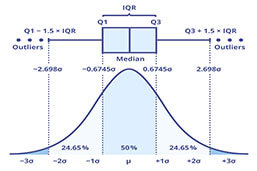
\includegraphics[width=0.9\textwidth]{./MP__boxplot.jpg}
\end{minipage}
    \caption{Interquartile range and boxplot}
    \label{fig:dp_iqr_boxpl}
\end{figure}

\section{Variable selection}
During the modelling process, the goal is to estimate a model, which shows the best performance on in-sample as well as out-sample data. While using all available information in the scoring function will lead to a high discriminatory power on the trained sample, usually result to multiple variables showing insignificant coefficients, meaning the p-value is below the confidence level and the null hypothesis that the coefficient = 0 cannot be rejected. This would also mean, that the confidence level may be too wide and the sign of the coefficient might be incorrect. Therefore, the model will likely show a worse performance on a different data set, as well as on the newest data, leading to unstable predictions. This problem is handled by considerate selection of variables depending on their discriminatory power, correlation and expert judgement. 

\subsection{Univariate Analysis}
All available variables should be considered for the modelling process. Then the missing rate, number of outliers and plausible values is assessed. If the variable complies with all data quality requirements, the discriminatory power will be determined. This can be performed using the univariate Gini coefficient or Information value, a more detailed explanation for both measures are in chapter \ref{sec:gini} and \ref{sec:dataprep}. The remaining risk factors with satisfying discriminatory power make up the long list. Example thresholds for each measure are:
\begin{itemize}
	\item \textbf{Missing rate}: < 20\%
	\item \textbf{Number of outliers}: < 5\%
	\item \textbf{Gini coefficient}: > 10\%
 	\item \textbf{Information value}: > 4\%
	\item \textbf{Correlation coefficient}: < 25\%
	\item \textbf{Variance Inflation Factor}: 5
\end{itemize}

\subsection{Multivariate Analysis}
The model variables should not be highly correlated because this can lead to multicollinearity issues and therefore in unstable coefficient estimates in the modelling process. Correlation between two variables can be measured using the Pearson or Spearman correlation coefficient (Eq. \ref{eq:dp_pears}, \ref{eq:dp_spear}). The Pearson correlation coefficient is more appropriate if a linear relationship is present. Spearman correlation coefficient is able to detect non-linear, monotonic interactions and is also more robust against outliers. The coefficient ranges from -1 (perfect negative correlation) to 1 (perfect positive correlation), with 0 indicating no correlation. After calculating all coefficients between each variable pair, all values can be arranged to a correlation matrix. An example is visible in Fig. \ref{fig:dp_corrmatrix}. 

\begin{equation}
\hat{\rho} = \frac{\sum_{i=1}^{n} (x_i - \hat{y}_X)(y_i - \hat{y}_Y)}{\sqrt{\sum_{i=1}^{n} (x_i - \hat{x}_X)^2 \sum_{i=1}^{n} (y_i - \hat{y}_Y)}} \label{eq:dp_pears}
\end{equation}
where:
\begin{conditions}
 x_i, y_i     				& individual observations \\
 \hat{y}_X, \hat{y}_Y    	& sample mean of X and Y  \\
 n    						& number of paired observations
\end{conditions}

\begin{equation}
\rho_s = 1 - \frac{6 \times \sum d_i^2}{n \times (n^2 - 1)} \label{eq:dp_spear}
\end{equation}
where:
\begin{conditions}
 d_{i}  & difference between the ranks of corresponding observations \\
 n    	& number of paired observations
\end{conditions}

\begin{figure}[H]
	\centering
	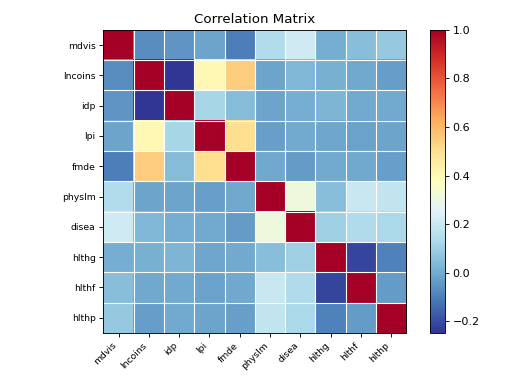
\includegraphics[width=0.625\textwidth]{./MP__corrmatrix.png}
    \caption{Correlation matrix example}
    \label{fig:dp_corrmatrix}
\end{figure}

If two variables are highly correlated with a correlation coefficient above a certain threshold, the variable with the lower discriminatory power should be removed from the model list. For categorical variables, the correlation statistic Variance Inflation Factor (VIF) can be utilised (Eq. \ref{eq:dp_vif}), which measures the collinearity in the regression analysis. Finally, adjustments based on expert judgement should be applied, where disqualified variables are forced into the list or variables, even if they meet all requirements, are removed. Especially the relationship between the explanatory factor and default rate should be analysed. If the behaviour contradicts the economic reasoning or experience, the variable should be eliminated from the model list, also called short list. 

\begin{equation}
\text{VIF}_{i} = \frac{1}{1 - R_{i}^2} \label{eq:dp_vif}
\end{equation}
where:
\begin{conditions*}
 R_{i}^2  & coefficient of determination obtained by regressing the i-th regressor on all the other regressors
\end{conditions*}

Example thresholds for the mentioned measures are:
\begin{itemize}
	\item \textbf{Correlation coefficient}: < 25\%
	\item \textbf{Variance Inflation Factor}: 5
\end{itemize}


\section{Modelling steps}
After selecting the most promising key factors, there are different approaches to determine the final model variables - the forward, backward, forward stepwise and backward stepwise selection procedure. In the first approach there are no variables in the model at the beginning and step by step the variable with the highest discriminatory power is added if the coefficient is significant (p-value below threshold). This step is repeated until no variable meets the condition. In the backward selection procedure, all variables are put into the model and then removed one by one depending on the coefficients' p-value, until all coefficients left in the model are significant. The forward stepwise procedure is a combination of both, where the model is first empty and variables are added successively, but after each addition, variables, which became insignificant, will be removed and the backward stepwise procedure is the opposite process. An procedures are illustrated in Figure \ref{fig:dp_fw_bw_proc} - \ref{fig:dp_fw_bw_step_proc}.

\section{Rating grades}
It is common to group the PDs into different rating bands such as investment and non-investment grade. The simplest approach is to use fixed ranges per grade. Another approach is to define PD intervals. An example is displayed in Fig. \ref{fig:dp_ratgrade}.